\documentclass{lug}

\title{Booting Linux}
\author{Jack Rosenthal}
\institute{Mines Linux Users Group}

\usepackage{etoolbox}

\makeatletter
\patchcmd{\beamer@sectionintoc}{\vskip1.5em}{\vskip0.5em}{}{}
\makeatother

\begin{document}

\begin{frame}{Table of contents}
    \setbeamertemplate{section in toc}[sections numbered]
    \tableofcontents[hideallsubsections]
\end{frame}

\section{Master Boot Record}

\begin{frame}{Floppy Disks}
    \begin{columns}
        \begin{column}{0.7\textwidth}
            \begin{itemize}[<+->]
                \item Floppy disks organized into 512-byte sectors
                \item Intel 8086 originally only allowed booting from floppy
                \item First sector is the \textbf{boot sector}, 512 bytes of
                    executable x86 machine code which runs in \textbf{real
                    mode}.
            \end{itemize}
        \end{column}
        \begin{column}{0.3\textwidth}
            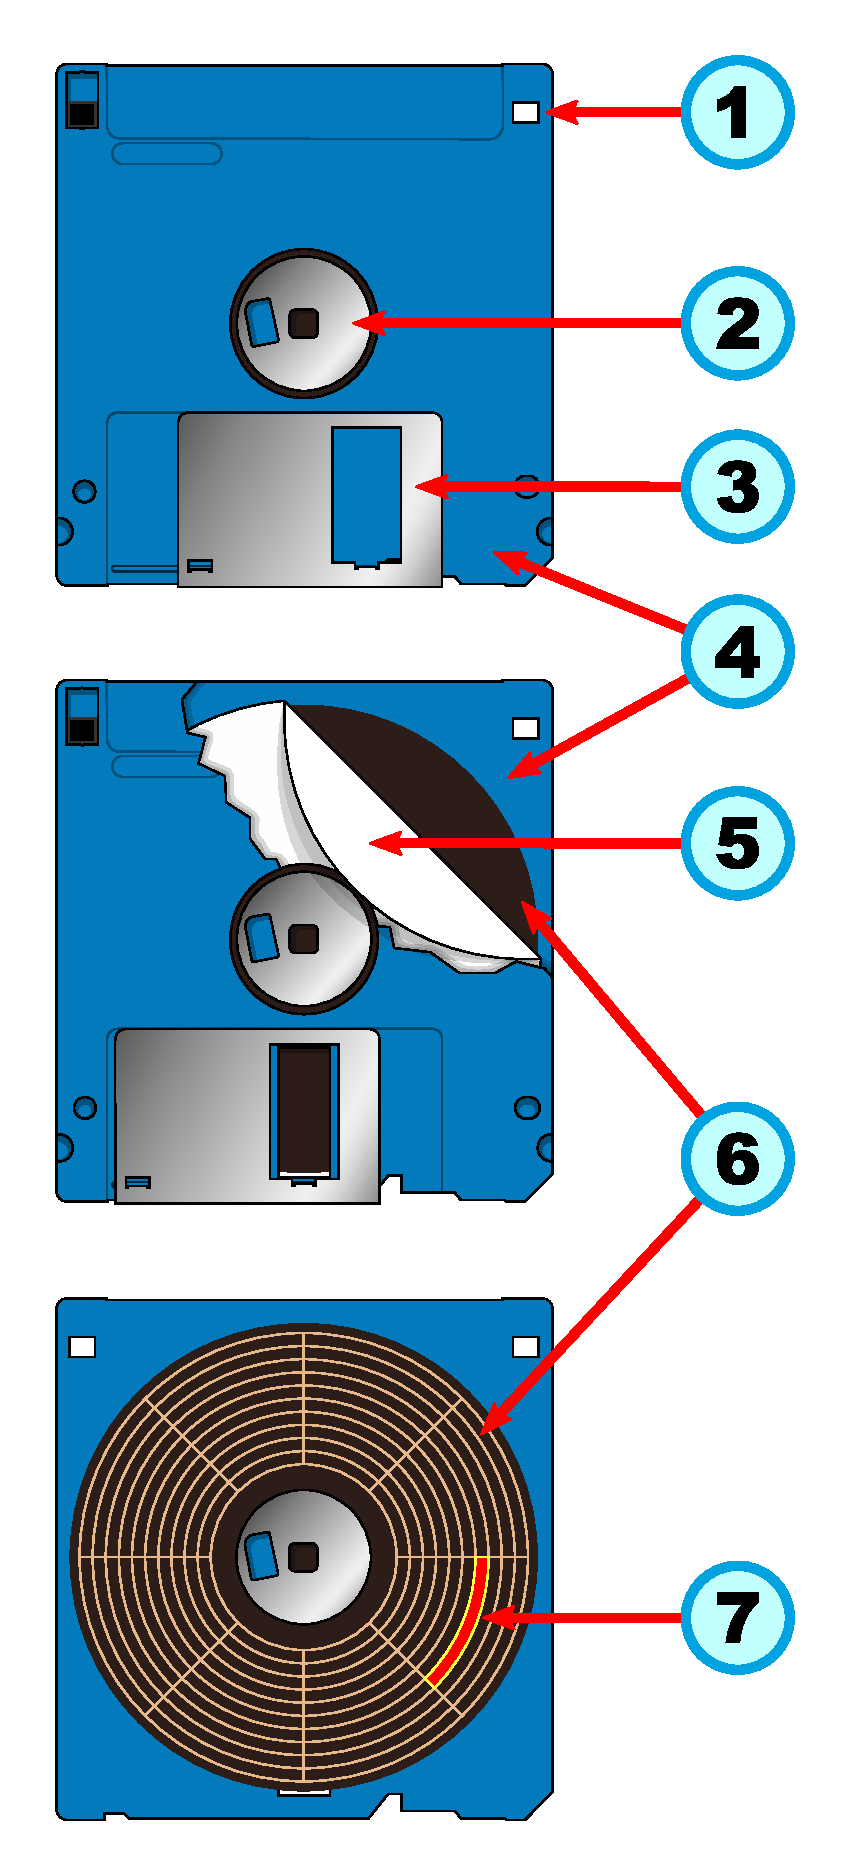
\includegraphics[width=\textwidth]{graphics/floppy_inside}
        \end{column}
    \end{columns}
\end{frame}

\begin{frame}{The 10 MB Hard Disk Came}
    \begin{columns}
        \begin{column}{0.7\textwidth}
            \begin{itemize}[<+->]
                \item IBM wanted a way to boot their systems off their new 10 MB hard
                    disk in 1983
                \item They added a 4-partition table to the end of the 512-byte boot
                    sector
                \item Boot sectors compatible with older systems because the machine
                    code ends before the partition data
                \item This is called \textbf{Master Boot Record}
            \end{itemize}
        \end{column}
        \begin{column}{0.3\textwidth}
            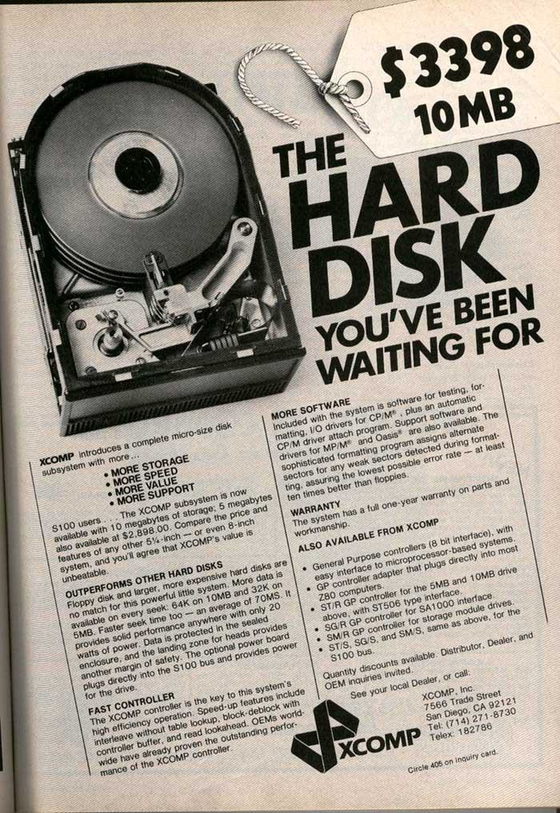
\includegraphics[width=\textwidth]{graphics/10mb}
        \end{column}
    \end{columns}
\end{frame}

\begin{frame}{Master Boot Record}
    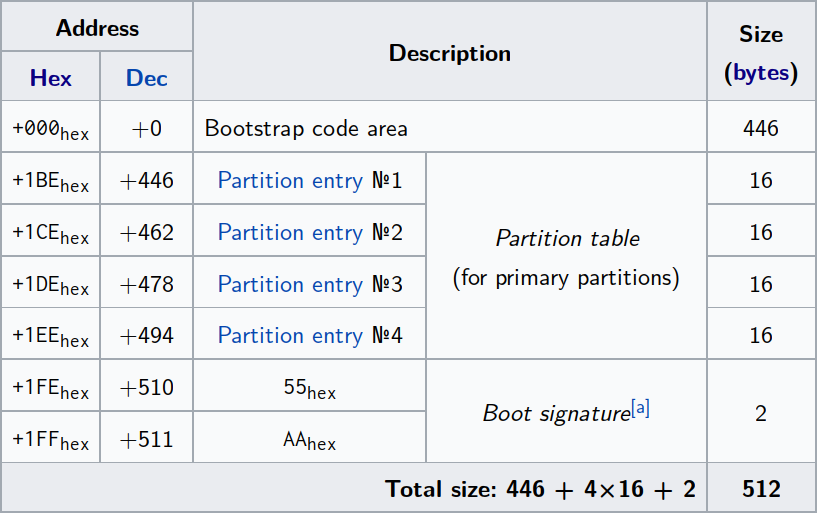
\includegraphics[width=\textwidth]{graphics/mbr_table}
\end{frame}

\begin{frame}{What does a MBR bootloader do?}
    \begin{enumerate}[<+->]
        \item Determine the partition to boot from
        \item Determine where your kernel image is on the partition
        \item Load the kernel into memory
        \item Enable protected mode
        \item Set up the environment for the kernel (stack space, etc.)
        \item Call your kernel's \texttt{main} function
    \end{enumerate}
    \pause[\thebeamerpauses]
    You will probably agree, that's a lot to do in 446 bytes of machine code.
\end{frame}

\begin{frame}{Some \emph{Real} Challenges}
    \begin{itemize}[<+->]
        \item Most C compilers won't compile to real mode code, so booting is
            on the \emph{list of things you can't even do in C}
        \item Real mode uses 16 memory segments of 64K each
        \item To switch segments, you must issue special instructions to the
            processor
        \item This gives you a total of 1 MiB of memory to use for booting
        \item \emph{Does your kernel fit in 1 MiB? Minus the memory you are
            using for your program to boot?}
    \end{itemize}
\end{frame}

\begin{frame}{Approaches to Solving Booting Challenges}
    \begin{itemize}[<+->]
        \item \textbf{Geek Booting:} Do everything your kernel needs to boot in
            the 512-byte boot sector. You will need your kernel to fit in 1 MiB
            as well. This is hard.
        \item \textbf{One-Stage Booting:} Write your bootloader in the first 1
            MiB of your kernel image, then write a 512-byte program that loads
            that program. The 1 MiB program is responsible for loading the rest
            of your kernel and booting it.
        \item \textbf{Two-Stage Booting:} Write a separate kernel that fits in
            1 MiB called a bootloader. This program is responsible for
            providing a high level interface to boot other kernels. GRUB is an
            example.
    \end{itemize}
\end{frame}

\section{Extensible Firmware Interface}

\begin{frame}{Apple}
    \begin{columns}
        \begin{column}{0.75\textwidth}
            \begin{itemize}[<+->]
                \item Historically, Macs have booted using a hardware chip on
                    the board called the \textbf{Macintosh ROM}
                \item The Mac ROM provided a miniature operating system (with a
                    mouse cursor and all) capable of booting Mac OS
                \item With the switch to PowerPC from 68K, Apple modified the
                    ROM to include an Open Firmware Interface capable of
                    extending booting capabilities beyond just classical Mac OS
            \end{itemize}
        \end{column}
        \begin{column}{0.25\textwidth}
            
\includegraphics[width=\textwidth]{graphics/happymac}
        \end{column}
    \end{columns}
\end{frame}

\begin{frame}{Apple}
    \begin{columns}
        \begin{column}{0.75\textwidth}
            \begin{itemize}[<+->]
                \item With the switch to Intel x86 from PowerPC, Apple looked
                    for a solution to boot Mac OS X from something that didn't
                    suck as much as MBR
                \item Apple looked at Intel's long forgotten \textbf{Extensible
                    Firmware Interface} (EFI)
                \item EFI was similar to Apple's OFI, but it worked on Intel
                    processors and had plenty of more features
                \item Thanks Apple! You popularized EFI and made booting x86
                    suck less!
            \end{itemize}
        \end{column}
        \begin{column}{0.25\textwidth}
            
\includegraphics[width=\textwidth]{graphics/happymac}
        \end{column}
    \end{columns}
\end{frame}

\begin{frame}{UEFI in a Nutshell}
    \begin{columns}
        \begin{column}{0.7\textwidth}
            \begin{itemize}[<+->]
                \item Simply write your bootloader in C and leave a \texttt{.efi}
                    binary on the FAT32 formatted \textbf{EFI System Partition}, the
                    system's UEFI firmware takes care of running your program for you
                \item Provides high level interfaces to the graphical console,
                    hardware, disks, memory, and even network
                \item Capable of doing hash checks on your bootloader to ensure it was
                    not tampered with by a computer virus
            \end{itemize}
        \end{column}
        \begin{column}{0.3\textwidth}
            
\includegraphics[width=\textwidth]{graphics/uefi}
        \end{column}
    \end{columns}
\end{frame}

\begin{frame}{Hello World EFI-Style}
    \small
    \inputminted{c}{efi_hello_world.c}
\end{frame}

\section{Booting Linux}

\begin{frame}{So this is all great, how does Linux boot?}
    \begin{enumerate}[<+->]
        \item First, the compressed Linux kernel (\texttt{vmlinuz}) is loaded
            by the bootloader and started
        \item The Linux kernel then loads a file system called \texttt{initrd}
            into memory which contains just enough programs to mount your disk
            and load drivers
        \item The kernel flag \texttt{root} specifies where your root partition
            is located to be mounted
        \item Once the root partition is mounted, \texttt{/etc/fstab} is read
            to determine any other partitions to be mounted
        \item \texttt{/bin/init} is called
    \end{enumerate}
\end{frame}

\begin{frame}{So what is \texttt{/bin/init}?}
    \begin{itemize}[<+->]
        \item \texttt{init} is the process with PID 1; it is the super-parent
            process of every process started on your system
        \item If \texttt{init} were to die, the kernel would panic
        \item Historically, System V style \texttt{init} programs would start a
            shell script located at \texttt{/etc/rc} that then loads your
            programs and desktop environment
        \item Most \texttt{/etc/rc} files use modularized shell scripts under
            \texttt{/etc/rc.d} or \texttt{/etc/init.d} to start services
        \item Shell scripts are \emph{slow}, and all sorts of standards exist
            for how to write these shell scripts
    \end{itemize}
\end{frame}

\begin{frame}{systemd: An alternative \texttt{init}}
    \begin{itemize}[<+->]
        \item Theory: Shell scripts as a configuration file is clunky and
            provides scattered interfaces
        \item Acts as a replacement \texttt{/bin/init} but uses configuration
            files rather than shell scripts
        \item This topic kind of deserves a talk of it's own? Anyone want to do
            it?
    \end{itemize}
\end{frame}

\section{Resources}

\begin{frame}{Resources}
    \begin{itemize}[<+->]
        \item \textbf{OSDev Wiki:} Great resource on developing your own OS,
            including writing bootloaders. \url{http://osdev.org}
        \item There's nothing else. That wiki has about everyting you need.
    \end{itemize}
\end{frame}

\begin{frame}[standout]
    \Huge
    Questions?
\end{frame}

\end{document}
